\documentclass[a4j]{jarticle}

\title{計算科学レポート1}
\author{学籍番号35-196004 天野智仁 }
\date{}

\usepackage{listings} %ソースコードの表示用
\usepackage[dvipdfmx]{graphicx}	% required for `\includegraphics' (yatex added)
\lstset{
  basicstyle={\ttfamily},
  identifierstyle={\small},
  commentstyle={\smallitshape},
  keywordstyle={\small\bfseries},
  ndkeywordstyle={\small},
  stringstyle={\small\ttfamily},
  frame={tb},
  breaklines=true,
  columns=[l]{fullflexible},
  numbers=left,
  xrightmargin=0zw,
  xleftmargin=3zw,
  numberstyle={\scriptsize},
  stepnumber=1,
  numbersep=1zw,
  lineskip=-0.5ex
}
\begin{document}
\maketitle
\section{AlのバンドとDOSの計算}
\subsection{DOS計算}
AlのDOSの計算の為に,まずはscf計算を行った.excercise1では,ファイルAl.sample.inによるscf計算で最適なdegaussとnkの値を求める.Al.sample.inはソースコード\ref{1}に与えられている.

\begin{lstlisting}[caption=Al.sample.in,label=1]
 &control
    calculation = 'scf',
    verbosity = 'high'
    prefix = 'Al_exc1'
    outdir = './tmp/'
    pseudo_dir = '../pseudo/'
 /
 &system
    ibrav =  2,
    celldm(1) = 7.65,
    nat =  1,
    ntyp = 1,
    ecutwfc = 25.0,
    occupations = 'smearing',
    smearing = 'marzari-vanderbilt',
    degauss = 0.02
 /
 &electrons
    mixing_beta = 0.7
 /

ATOMIC_SPECIES
 Al 26.98  Al.pz-vbc.UPF

ATOMIC_POSITIONS (alat)
 Al 0.0 0.0 0.0

K_POINTS (automatic)
  8 8 8 1 1 1 
\end{lstlisting}

結晶はprimitive cellの原点に一つだけAlを含むFCC構造である.これは実際にxcrysdenで図示することができて,下図\ref{040724_19May19}のようになる.
 \begin{figure}[htb]
  \begin{center}
   \includegraphics[width=5cm]{pwi2xsf.png}
   \caption{Alの結晶構造}
   \label{040724_19May19}
   \end{center}
 \end{figure}


degaussとnkに対する繰り返し計算は,$k=6,78,12,16$および$degauss=0.02$から$0.02$刻みで$0.10$までで行った.その結果は図\ref{050705_19May19}に示されている.
degaussの性質から,degaussは小さい程正確な基底エネルギーを与えられると考えられるが,図\ref{050705_19May19}はこの様子を反映して,基底エネルギーがdegaussに関する単調増加の関数になっている.一方でnkは大きいほど良いが,degaussが$0.02$の時の値を見て見ると,nkは8でも既に16の時の値と高い精度で一致しており,計算量低減の為にもnkは8で計算することにした.scf計算によって得られたTotal Energyは$-4.18867883 Ry$,Fermi Energyは$7.6495 ev$ である.
\begin{figure}[htb]
 \begin{center}
  \includegraphics[bb=0 0 640 480,width=10cm]{Al.TotalEnergy.png}
  \caption{degaussに関する繰り返し計算}
  \label{050705_19May19}
 \end{center}
\end{figure}


この結果を用いて,nscfの計算を行った.nscf計算を行う際のscfからの変更点を図にまとめた.
\begin{lstlisting}
 &CONTROL
 calculation='nscf'

 &SYSTEM
 occupations='tetrahedra'

 &K_POINTS
 16 16 16 1 1 1
\end{lstlisting}
nkをscf計算の時の2倍に増やす理由は,より細かいk点での計算を行うためである.


これらを元に,DOSの計算を行う.DOSの計算はFermi Energyを基準にとって図\ref{035614_19May19}に図示した.
\begin{figure}[htb]
 \begin{center}
  \includegraphics[width=10cm]{Al.dos.eps}
  \caption{AlのDOS図}
  \label{035614_19May19}
 \end{center}
\end{figure}

また電荷密度の計算も行い,conventional cellの一面について図\ref{054539_19May19}に示した.
\begin{figure}[htb]
 \begin{center}
  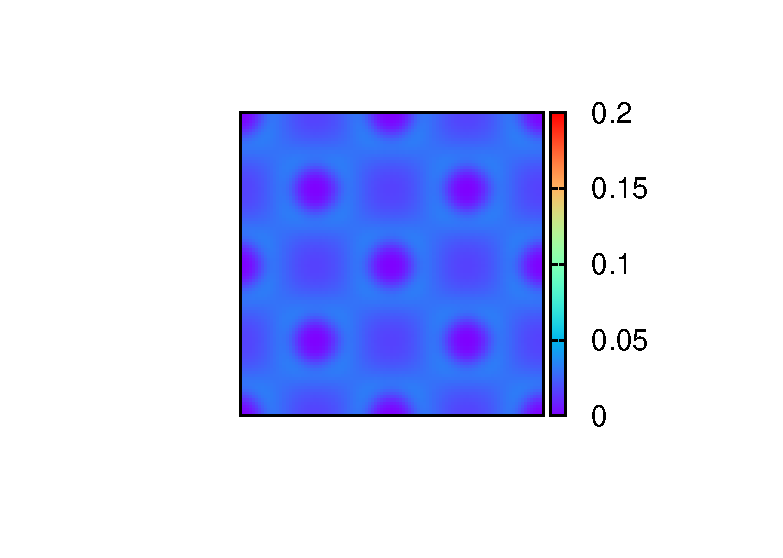
\includegraphics[width=7cm]{charge.eps}
  \caption{Alの電荷密度}
  \label{054539_19May19}
 \end{center}
\end{figure}
\newpage


\subsection{bandsの計算}
bandの計算にも,DOSと同じscf計算の結果を用いた.すなわちdegaussは0.02,kメッシュは8である.nscf計算をband計算用に実行し直す.変更点を図にまとめた.

\begin{lstlisting}
 &control
 calculation = 'bands'

 K_POINTS{tpiba_b}
 6
 gG 30
 X  30
 W  30
 L  30
 gG 30
 K  30
\end{lstlisting}

この計算を元に得られたband図が,図\ref{033638_19May19}である.ただし基準をフェルミ面にとってある.
\begin{figure}[htb]
 \begin{center}
  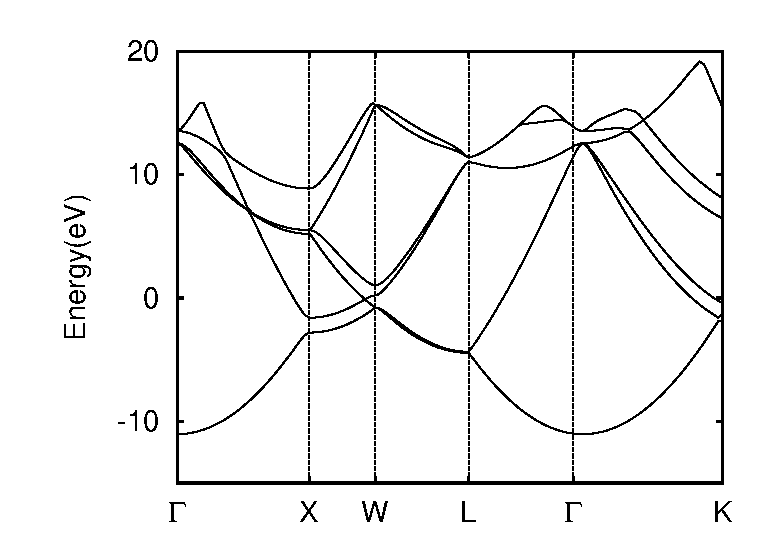
\includegraphics[width=10cm]{Al.bands.eps}
  \caption{Alのバンド図}
  \label{033638_19May19}
 \end{center}
\end{figure}
バンド図を見ればわかるようにAlは金属である.K-pathの取り方は図\ref{044438_19May19}に示されている通りである.

\begin{figure}[htb]
 \begin{center}
  \includegraphics[width=5cm]{Al.Kpath2}
  \caption{K-pathの取り方}
  \label{044438_19May19}
 \end{center}
\end{figure}
\newpage


\section{Cuのバンド計算}

Cuのバンド計算もAlと同様に行う.CuはAlと同じFCC構造であるから,原子の種類をAlからCuに変更し(同時に擬ポテンシャルも変更する)格子定数を変更するだけで系の設定は十分である.それに加えて設定上の問題から,prefixも変更した.
 \begin{lstlisting}
  &CONTROL
  prefix = 'Cu_exc3'
  
  &SYSTEM
  a = 3.61496
  
 &ATOMIC_SPECIES
  Cu 63.546 Cu.pz-d-rrkjus.UPF 
 \end{lstlisting}

 まず初めのdegaussとnkに関する繰り返し計算の結果が図\ref{052122_19May19}である.今回も同様に,degaussを$0.02$,nkを$8$で計算すれば十分であろう.また,この時の全エネルギー
 $-87.85031985 Ry$,フェルミエネルギーは$13.6131 ev$であった.
 
 \begin{figure}[htb]
  \begin{center}
   \includegraphics[bb=0 0 640 480,width=10cm]{CuTotalEnergy.png}
   \caption{degaussの繰り返し計算}
   \label{052122_19May19}
  \end{center}
 \end{figure}

 次にband計算のためのnscf計算を行い,バンド図\ref{035904_19May19}を得た.バンド図においてフェルミエネルギーの下を占めている多数のバンドはd電子由来のバンドであり,Cuの特徴がよく捕らえられているといえる.
 
 \begin{figure}[htb]
  \begin{center}
   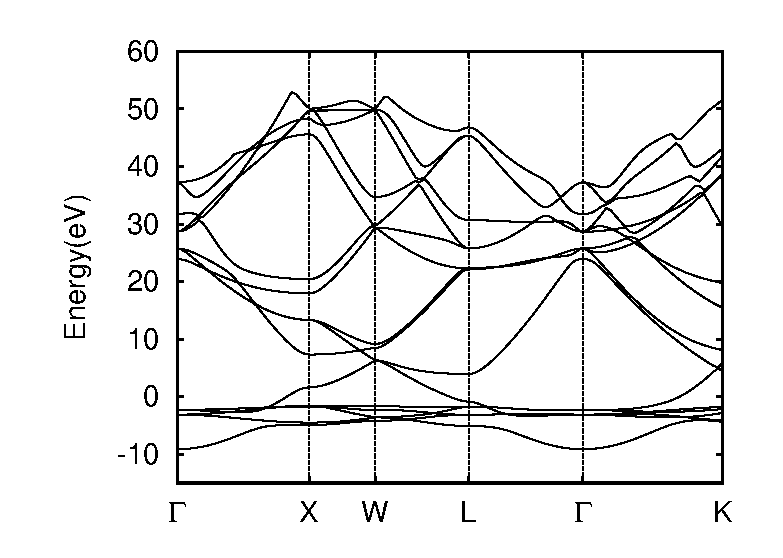
\includegraphics[width=10cm]{Cu.bands.eps}
   \caption{Cuのバンド図}
   \label{035904_19May19}
   \end{center}
 \end{figure}



\end{document}